\section{Auswertung}
\label{sec:Auswertung}

%Aufgabe 1
Nach \autoref{sec:durchfuehrung} wird der Versuch aufgebaut und für $7$ verschiedene Einfallswinkel $\alpha_1$ der Reflexionswinkel $\alpha_2$
bestimmt. Als Grenzfläche wird hierbei ein Spiegel genutzt. Die ermittelten Werte werden in \autoref{tab:Reflexion} dargestellt.
\begin{table}
  \centering
  \caption{Verifizierung des Reflexionsgesetzes.}
  \label{tab:Reflexion}
  \sisetup{table-format=2.2}
  \begin{tabular}{S S}
  \toprule
  {Einfallswinkel $\alpha_1$} &{Reflexionswinkel $\alpha_2$}\\
  \midrule
  20 & 20 \\
  30 & 30 \\
  35 & 35 \\
  40 & 40 \\
  45 & 45 \\
  50 & 50 \\
  60 & 60 \\
  \bottomrule
  \end{tabular}
\end{table}

Durch die Messung der Einfalls- und Ausfallswinkel lässt sich das Reflexionsgesetz verifizieren.
Die Genauigkeit der Winkel ist jedoch durch menschliche Ablesefehler eingeschränkt. Außerdem ist die Skala in 1 Grad Schritte aufgeteilt,
sodass eine genauere Bestimmung der Winkel darüber hinaus sehr schwierig ist.

%Aufgabe 2

Der Versuchsaufbau wird nun so abgeändert, dass der Laser auf eine planparallele Platte trifft. Es wird für 7 verschiedene
Einfallswinkel $\alpha$ der Brechungswinkel $\beta$ bestimmt und in \autoref{tab:Brechung} aufgetragen. Zudem wird aus diesen Werten
der Brechungsindex $n$


\begin{figure}
  \centering
  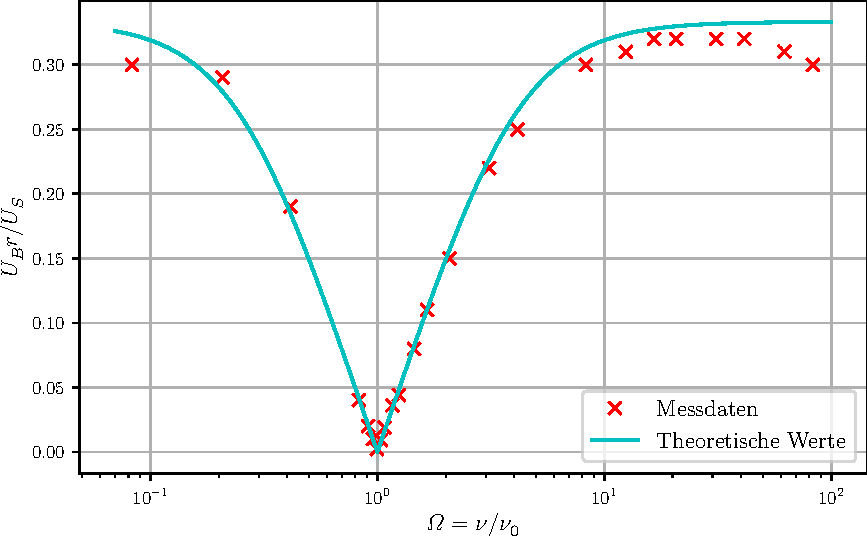
\includegraphics{plot.pdf}
  \caption{Plot.}
  \label{fig:plot}
\end{figure}


Siehe \autoref{fig:plot}!
